Our analysis of the CPU capabilities so far has shown that the processor can execute multiple operations at once as long as the operands are already in the registers: we can evaluate a fairly complex expression that depends on just two values in exactly as much time as it takes to add these values. The depends on just two values qualifier is, unfortunately, a very serious restriction. We now consider a more realistic code example, and we don't have to make many changes to our code:

\begin{lstlisting}[style=styleCXX]
for (size_t i = 0; i < N; ++i) {
	a1 += (p1[i] + p2[i])*(p1[i] - p2[i]);
}
\end{lstlisting}

Recall that the old code had the same loop with a simpler body: a1 += (p1[i] + p2[i]);. Also, p1[i] is just an alias for the vector element v1[i], same for p2 and v2. Why is this code more complex? We have already seen that the processor can do addition, subtraction, and multiplication in a single cycle, and the expression still depends on just two values, v1[i] and v2[i]. However, this expression cannot be evaluated in one cycle. To clarify this, we introduce two temporary variables that are really just names for the intermediate results during expression evaluation:

\begin{lstlisting}[style=styleCXX]
for (size_t i = 0; i < N; ++i) {
	s[i] = (p1[i] + p2[i]);
	d[i] = (p1[i] - p2[i]);
	a1[i] += s[i]*d[i];
}
\end{lstlisting}

The results of the addition and the subtraction, s[i] and d[i], can be evaluated at the same time, as we saw earlier. However, the last line cannot be executed until we have the values of s[i] and d[i]. It doesn't matter how many additions and multiplications the CPU can do at once: you cannot compute the result of an operation whose inputs are unknown; therefore, the CPU has to wait for the inputs to the multiplication to become ready. The i-th iteration has to be executed in two steps: first, we have to add and subtract (we can do both at once), and second, we have to multiply the results. The iteration now takes two cycles instead of one because the second step of the computation depends on the data produced by the first step:

\hspace*{\fill} \\ %插入空行
\begin{center}
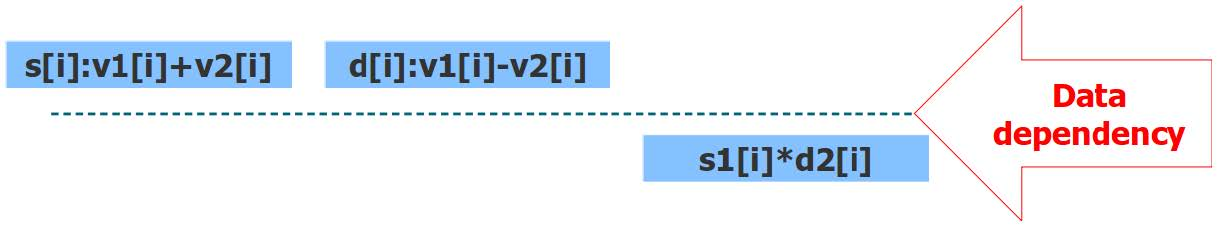
\includegraphics[width=0.9\textwidth]{content/1/chapter3/images/14.jpg}\\
Figure 3.14 – Data dependency in loop evaluation
\end{center}

Even though the CPU has the resources to do all three operations at once, we cannot take advantage of this capability because of the data dependency inherent in our computations. This, of course, severely limits how efficiently we can use our processor. Data dependencies are very common in programs, but fortunately, the hardware designers came up with an effective antidote. Consider Figure 3.14 carefully. We have the multiplication hardware unit standing by idly while we compute the values of s[i] and d[i]. We cannot start computing their product any earlier, but there is something else we can do: we can multiply the values s[i-1] and d[i-1] from the previous iteration at the same time. Now the two iterations of the loop are interleaved in time:

\hspace*{\fill} \\ %插入空行
\begin{center}
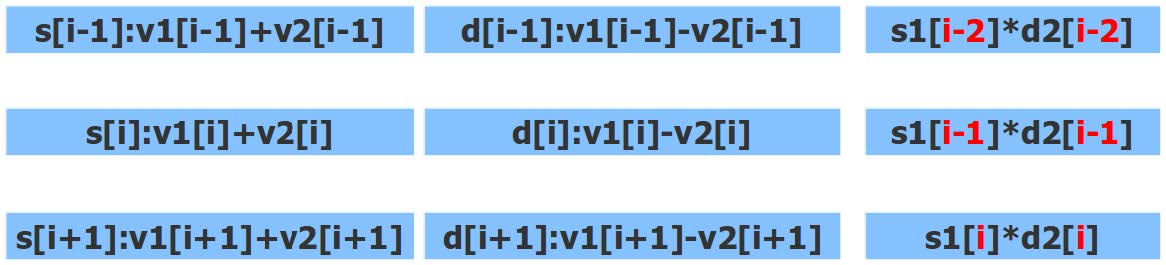
\includegraphics[width=0.9\textwidth]{content/1/chapter3/images/15.jpg}\\
Figure 3.15 – Pipelining: the rows correspond to the successive iterations; all operations in the same row are executed simultaneously
\end{center}

This transformation of the code is known as pipelining: a complex expression is broken up into stages and executed in a pipeline where stage 2 of the previous expression runs at the same time as stage 1 of the next one (a more complex expression would have more stages and require a deeper pipeline). If we are correct in our expectations, the CPU will be able to compute our two-stage add-subtract-multiply expression just as fast as single multiplication as long as we have many iterations: the first iteration is going to take two cycles (add/subtract first, then multiply), there is no getting around that. Similarly, the last iteration will end with a single multiplication, and there is nothing else we can do at the same time. However, all the iterations in between will be executing three operations simultaneously. We already know that our CPU can add, subtract, and multiply at the same time. The fact that the multiplication belongs to a different iteration of the loop matters not at all.

We can confirm our expectations with a direct benchmark, where we compare the time it takes to do one multiplication per loop iteration with the time it takes to do our two-step iteration:

\hspace*{\fill} \\ %插入空行
\begin{center}
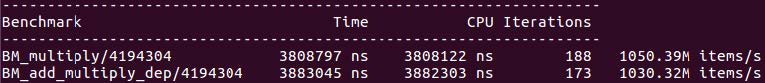
\includegraphics[width=0.9\textwidth]{content/1/chapter3/images/16.jpg}\\
Figure 3.16
\end{center}

As expected, both loops run at essentially the same speed. We can conclude that the pipelining has completely negated the performance penalty caused by the data dependency. Note that the pipelining does not eliminate the data dependency; each loop iteration still has to be executed in two stages, with the second stage depending on the results of the first one. However, by interleaving the computations from different stages, the pipelining does eliminate the inefficiency that would be otherwise caused by this dependency (at least in the ideal case, which is what we have so far). An even more direct confirmation can be seen in the results of the Machine Code Analyzer. Again, the timeline view is the most instructive:

\hspace*{\fill} \\ %插入空行
\begin{center}
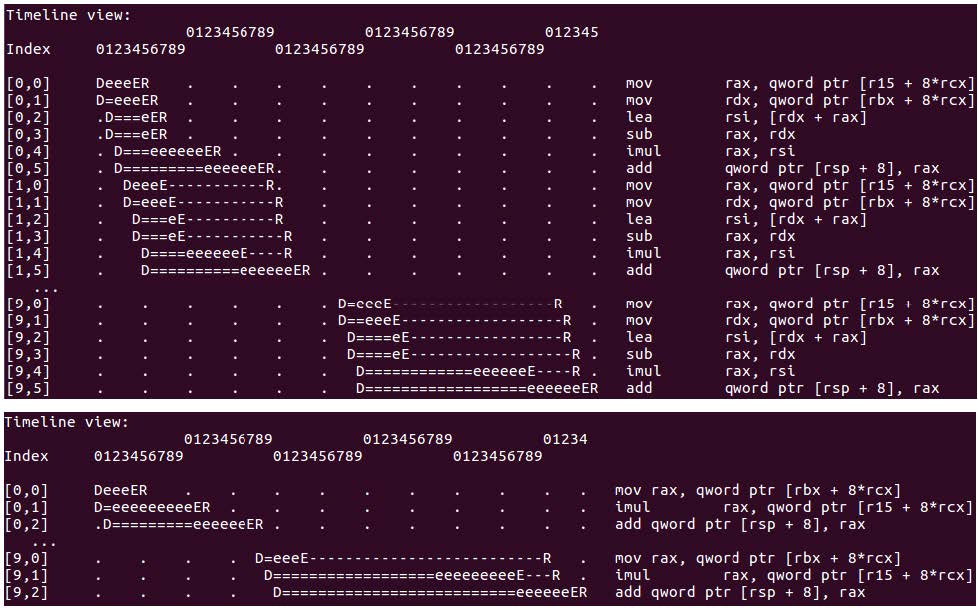
\includegraphics[width=0.9\textwidth]{content/1/chapter3/images/17.jpg}\\
Figure 3.17 – A timeline view of the pipelined add-subtract-multiply loop (top) vs. a loop with a single multiplication (bottom)
\end{center}

As you can see, it takes 56 cycles to execute ten iterations of either loop. The key step in the timeline is when an instruction is executed: e marks the beginning of the execution, and E is when the execution ends. The effect of the pipelining is clearly visible in the timeline: the first iteration of the loop starts to execute on the second cycle with the instruction [0,0]; the last instruction of the first iteration is done executing on cycle 18 (the horizontal axis is the cycle number). The second iteration begins executing on cycle 4, that is, there is a significant overlap of the two iterations. This is the pipelining in action, and you can see how it improves the efficiency of our program: at almost every cycle, the CPU is executing instructions from multiple iterations using its many computation units. It takes just as many cycles to execute a simple loop as it does to execute the more complex one, so the extra machine operations take no additional time.

This chapter is not intended to be a manual for the Machine Code Analyzer: to understand better the timeline and other information it produces, you should study its documentation. There is, however, one issue that we must point out. Every iteration of our loop does not just have the same C++ code, it has exactly the same machine code as well. This makes sense: the pipelining is done by the hardware, not the compiler; the compiler simply generates the code for one iteration and the operations needed to advance to the next iteration (or exit the loop upon completion). The processor executes multiple instructions in parallel; we can see that in the timeline. But something does not make sense upon close examination: for example, consider the instruction [0,4] in Figure 3.17. It is executed during cycles 6 through 12, and it uses registers CPU rax and rsi. Now look at the instruction [1,2] that is executed during cycles 8 and 9: it also uses the same registers, it actually writes into the register rsi, which is still being used by other instructions at the same time. This cannot be: while the CPU can do multiple operations simultaneously using its many independent computing units, it cannot store two different values in the same register at the same time. This contradiction was actually present, although well-hidden, all the way back in Figure 3.15: assuming that the compiler generates only one copy of the code for all iterations, the register we are going to use to store the value of s[i] is exactly the same as the one we need to read the value of s[i-1], and both actions happen at the same time.

It is important to understand that we are not running out of registers: the CPU has many more registers than we have seen named so far. The problem is that the code for one iteration looks exactly like the code for the next iteration, including the register names, but at each iteration, different values must be stored in the registers. It seems like the pipelining we have assumed and observed should not, in fact, be possible: the next iteration must wait for the previous iteration to stop using the registers it needs. This is not what really happens, and the solution to this apparent contradiction is the hardware technique called register renaming. The register names you see in the program, such as rsi, are not the real register names, they are mapped by the CPU to the actual physical registers. The same name, rsi, can be mapped to different registers that all have the same size and functionality.

When the processor executes the code in a pipeline, the instructions from the first iteration that refer to rsi will, in fact, use an internal register that we shall call rsi1 (this is not its real name, but the actual hardware names of registers are not something you would ever encounter unless you are designing a processor). The second iteration also has instructions that refer to rsi but needs to store a different value there, so the processor will use another register, rsi2. Unless the first iteration no longer needs the value stored in rsi, the third iteration will have to use yet another register, and so on. This register renaming is done by the hardware and is very different from the register assignment done by the compiler (in particular, it is entirely invisible to any tool that analyzes the object code, such as LLVM-MCA or a profiler). The end effect is that multiple iterations of the loop are now executed as a linear sequence of code as if s[i] and s[i+1] really did refer to different registers.

Converting a loop into linear code is known as loop unrolling; it is a popular compiler optimization technique, but this time, it is done in hardware and is essential to be able to deal with data dependencies efficiently. The compiler's point of view is closer to the way the source code is written: a single iteration, a group of machine instructions, executed over and over by jumping back to the beginning of the code fragment for the iteration. The processor's point of view is more like what you see in the timeline, a linear sequence of instructions where each iteration has its own copy of the code and can use different registers. 

We can make another important observation: the order in which the CPU executes our code is actually not the same order in which the instructions are written. This is called out-of-order execution, and it has important consequences for multi-threaded programs.

We have seen how the processor avoids the restrictions on the efficiency of execution that would be imposed by data dependencies: the antidote to the data dependency is the pipelining. However, the story does not end there, and the beautifully complex scheme we have devised so far to execute our very simple loop is missing something important: the loop must end at some point. In the next section, we will see how much that complicates things and what the solution is.























